%=========================================================================
%Jakub Bartecek (xbarte09)
%Date: 2013 - 2014
%Encoding: UTF-8
%set syntax=tex




\chapter{Úvod}
    Tento semestrální projekt se zabývá vylepšením serveru Jenkins CI, který je v praxi velmi využíván pro potřeby průběžného testování softwaru
    a jeho kontinuální integraci. Vylepšení se týká především webového serveru a \emph{servlet} kontejneru, který je v Jenkins CI integrován. 
    V současném stavu tyto funkce vykonává kombinace nástrojů Winstone a Jetty. 
    
    Server Winstone je již neudržovaný a zastaralý nástroj a z tohoto důvodu
    byl z velké části nahrazen serverem Jetty, který potřebnou funkcionalitu poskytuje. Server Jetty je poměrně komplexní projekt a nabízí
    mnoho funkcionality, ale na druhou stranu jeho rozsah nedovoluje poskytovat maximální rychlost.
    
    V současné době vznikl nový webový server Undertow, který si klade za cíl být co nejjednodušší a nejrychlejší a mohl by být přínosný
    a vhodný pro Jenkins CI. Jelikož tento server je nový a je sponzorován firmou Red Hat, tak lze předpokládat, že jeho vývoj
    bude nadále pokračovat a nebude zastarávat.

    Cílem této práce je nahradit server Jetty a případně i serveu Winstone pomocí serveru Undertow 
    a integrovat jej se serverem Jenkins CI. Při integraci je kladen důraz na snahu
    zachovat zpětnou kompatibilitu se starým řešením. 

    V rámci tohoto semestrálního projektu jsou nejprve rozebrány potřebné informace týkající se jednotlivých nástrojů a plánované integrace.
    Následně je detailně analyzována architektura Jenkins CI a způsob jeho integrace se servery Winstone a Jetty. V následující části
    je diskutována varianta nahrazení pouze serveru Jetty a varianta nahrazení serveru Jetty i Winstone pomocí serveru Undertow. 
    Z provedené analýzy je zvolena jedna varianta, která je vybrána pro následnou integraci.

    Samotná implementace integrace není předmětem tohoto semestrálního projektu a bude provedena až v navazujícím diplomovém projektu. 
    V rámci dimplomového projektu bude také provedeno testování výkonu modifikovaného systému Jenkins CI a celkové shodnocení navržených
    a provedených změn.
%TODO - že to dělám pod Red Hatem


\chapter{Jenkins CI a související nástroje}
    Tato kapitola se zaměřuje na teoretické základy práce, které je nutné nebo vhodné znát pro pochopení zpracovávané problematiky.
    Je zde detailněji popsán systém Jenkins CI (kapitola \ref{jenkins}) ke kterému se tato práce přímo váže. S ním je spojeno seznámení
    s webovými servery Winstone (kapitola \ref{winstone}) a Jetty (kapitola \ref{jetty}), jejichž kombinace je současně v Jenkins CI integrována.
    Pro tuto práci je důležité poruzumět rozdílu mezí \emph{servlet kontejnerem} a webovým server. Vysvětlením těchto pojmů se zabývá kapitola \ref{servletWebserver}.

    Větší důraz je dále věnován serveru Undertow (kapitola \ref{undertow}), který byl vybrán jako nový webový server pro Jenkins CI. V tomto případě je provedena hlubší studie
    tohoto nástroje, aby na jejím základě bylo možné pochopit a provést samotnou integraci s Jenkins CI, která je jádrem této práce. 
    Pro poskytnutí ucelených informací
    je menší prostor také vymezen pro nástroj Maven (kapitola \ref{maven}), který se používá k řízení překladu serveru Jenkins CI, a je v této práci několikrát zmiňován. 

    Uvedené informace mají spíše informativní charakter, aby poskytly ucelený úvod do zkoumané problematiky. Jsou zaměřeny především na informace týkající se samotné
    integrace. Pro případné získání detailnějších informací jsou uvedeny patřičné zdroje, kde je lze hledat.

    \section {Jenkins CI} \label{jenkins}
        Jenkins CI je komunitní open source nástroj pro kontinuální integraci softwaru, který je vyvíjen pod svobodnou licencí
        MIT\footnote{Licence MIT: http://opensource.org/licenses/MIT} \cite{jenkinsGovernance}.
        Je velmi populární a využíván malými i velkými firmami jako je například firma Red Hat, kde tento program běží na stovkách serverů.
        Původní název tohoto projektu je Hudson\footnote{Webové stránky projektu Hudson: http://hudson-ci.org/}. 
        Když se vývoje tohoto projektu ujala firma Oracle, tak se tento projekt
        rozštěpil a vznikla komunitní verze projektu, což je server Jenkins CI. Přesto se v některých částech tohoto projektu 
        stále objevuje název Hudson, ale jedná se pouze pozůstatek z původního projektu.

        Zkratka CI je z anglického spojení \emph{continuous integration}, což lze do češtiny přeložit jako kontinuální nebo průběžná 
        integrace. Krátké seznámení se z touto metodologií je v následující kapitole.

        Informace v této kapitole byly především čerpány z knihy \cite{jenkinsBook}, kde lze nalézt další informace o serveru Jenkins CI,
        a také z webové stránky projektu \cite{jenkinsWeb}.

        \subsection{Kontinuální integrace a využití Jenkins CI}
            V minulosti byla integrace programu do výsledného produktu velmi náročným procesem a často ztraceným časem.
            S vydáním každé verze programu se musel postup probíhající před vydáním produktu opakovat a pro vývojářský tým
            to prakticky znamenalo zdržení se. Pokud se v tomto procesu odhalil nějaký problém, což bylo běžné, 
            tak jeho řešení bylo z důvodu nedostatku času a jeho pozdního objevení mnohem problematičtější,
            než kdyby byl tento problém odhalen dříve.

            Kontinuální integrace je moderní přístup k vývoji softwaru, který mění způsob myšlení nad celým procesem vývoje
            a snaží se předcházet problémům popsaným výše a především ušetřit čas. V tomto přístupu je využíván nějaký
            kvalitní nástroj, který automatizovaně provádí specifikované kroky, které provázejí integraci softwaru a jeho vydání.

            Jedním z nástrojů poskytujích podporu pro kontinuální integraci při vývoji softwaru je 
            server Jenkins CI. 
            
            \medskip \noindent Základními možnostmi, které umožňuje Jenkins CI nakonfigurovat, jsou:
            
            \begin{itemize}
                \item Spouštění integračních a jednotkových testů v přesně definovaném čase (např. v noci, kdy jsou servery méně vytížené)
                \item Spuštění integračních a jednotkových testů při změně ve verzovacím systému. Jenkins CI dokáže zaznamenat změnu v repozitáři,
                    stáhnout si změny a spustit testování
                \item Shromažďování a vyhodnocování metrik vývoje softwaru
                \item Spuštění akceptačních testů
                \item Informování e-mailem o testech, které skončily chybou
                \item Automatické nahrání nové verze produktu na server
            \end{itemize} 

            Uživatelé mohou kdykoliv přidat využití libovolné funkcionality systému a tudíž neopakovat stále stejné kroky. 
            

        \subsection{Způsoby použití aplikace}
            Celý program je napsán v jazyce Java a je tedy plně přenositelný mezi platformami. Architektura je navržena tak, aby byla 
            lehce rozšiřitelná pomocí tzv. \emph{pluginů}, kterých je pro Jenkins vytvořené velké množství. 
            
            Jenkins CI je určen pro běh na serveru a je dostupný přes webové rozhraní (ale může být samozřejmě spuštěn
            na libovolném osobním počátači). Komunikuje pomocí protokolu \emph{HTTP}, 
            který je založen na modelu \emph{požadavek-odpověď} (anglicky \emph{request-response}). Jelikož tento způsob komunikace
            je velmi běžný, tak není v programu přímo implementován, ale využívá k němu externí nástroje. 
            Dalším nástrojem, který pro svou činnost Jenkins potřebuje, je servlet kontejner ve kterém samotná 
            aplikace poběží.
            Tento pojem je blíže objasněn v kapitole \ref{servletWebserver}.

            \medskip \noindent
            Existují dvě možnosti jak spustit server Jenkins CI:

            \begin{enumerate}
                \item{Může běžet na libovolném \emph{Java EE} aplikačním serveru \cite{jenkinsServers} jako jsou například servery 
                JBoss\footnote{Více informací o serveru viz http://www.jboss.org/jbossas/} 
                anebo Glasfish\footnote{Více informací o serveru viz http://www.oracle.com/technetwork/middleware/glassfish/}}.
                Jenkins CI se standardně nasadí na server (dle zvyklostí konkrétního serveru)
                a poté je s ním možné pracovat. V tomto případě veškerou nízkoúrovňovou komunikaci pomocí \emph{HTTP} 
                i práci servlet kontejneru zajišťuje aplikační server.
                
                \item{Pokud nechceme nebo nemůžeme spouštět Jenkins CI na aplikačním serveru, tak jej lze spustit přímo
                    z vytvořené \texttt{.war} archivu (překladem se zabývá kapitola \ref{jenkinsUsage}). V tomto případě
                    se o práci servlet kontejneru i webového serveru komunikujícího protokolem \emph{HTTP} stará 
                    kombinace nástrojů Winstone a Jetty, které jsou přímo integrovány do serveru Jenkins CI. 
                    
                    Nahrazení těchto dvou nástrojů (nebo pouze serveru Jetty) a zajištění vykonávání této činnosti je hlavním cílem této práce.
                    Záměrem je tedy nahradit server Jetty a případně i server Winstone pomocí zvoleného nového serveru Undertow.
                    Studie těchto nástrojů a jejich rozbor je předmětem následujícíh kapitol.}
            \end{enumerate}

            Pro tuto práci je důležitý druhý způsob používání Jenkins CI a proto další informace se budou přímo vázat k němu.

        \subsection{Základy práce s Jenkins CI} \label{jenkinsUsage}
            Pro přeložení a spuštění aplikace je potřeba pracovat z příkazové řádky nebo provést instalaci nějakým dávkovým souborem (skriptem).
            Aplikaci je možné stáhnout připravenou přímo ze stránek projektu \cite{jenkinsWeb}, ale pro tuto práci je potřeba 
            pracovat s aplikací ze zdrojových souborů. Aktuální verze aplikace je dostupná na serveru 
            GitHub\footnote{Adresa aktuální verze Jekins CI: www.github.com/jenkinsci}.

            Po stažení zdrojových souborů je potřeba provést překlad aplikace. Pro tento automatizovaný překlad se používá nástroj Maven, který
            krátce zmíněn v kapitole \ref{maven}. Pro provedení překladu bez spouštění jednotkových testů je potřeba použít tento příkaz:
            \begin{verbatim}
                mvn clean install -pl war -am -DskipTests
            \end{verbatim}
            Pokud bychom chtěli spustit jednotkové testy aplikace, tak jednoduše vynecháme poslední přepínač. Nejjednodušším 
            způsobem kontroly provedených změn v programu je právě spouštění automatizovaných testů a proto je tato možnost
            velmi důležitá pro plánovanou integraci se serverem Underotw. Kromě jednotkových testů obsahuje Jenkins CI také
            integrační testy, které jdou více do hloubky aplikační logiky a jsou schopny odhalit větší množství chyb, 
            ale na druhou stranu jejich vykonání trvá dlouhou dobu (řádově více než hodinu). Integrační testy lze spustit
            příkazem:
            \begin{verbatim}
                mvn clean package
            \end{verbatim}
            Další nevýhodou integračních testů je, že je běžný stav, kdy některé testy, aplikace která je překládaná z aktuálních zdrojových souborů,
            končí s chybou. Proto je při kontrole nutné porovnávat výsledky testů před provedením změn a po jejich provedením. Tento způsob
            kontroly aplikace bude využit při hodnocení navazující diplomové práce.

            \medskip
            Po úspěšnm překladu aplikace vznikne v adresáři \texttt{./war/target/} archiv \texttt{jenkins.war}, 
            který obsahuje celou přeloženou webovou aplikaci včetně nástrojů na 
            kterých závisí. Z tohoto archivu je možné aplikaci přímo spustit pomocí příkazu:

            \begin{verbatim}
                java -jar jenkins.war
            \end{verbatim}
            Je možné nastavit ještě další parametry při spuštění programu, které lze vypsat pomocí přidání parametru \texttt{--help}.

            Pro práci se spuštěnou instancí aplikace se používá především webové rozhraní. Standardně aplikace
            komunikuje pomocí protokolu \emph{TCP} na portu 8080. Je tedy možné se na lokálním počítači připojit do aplikace zadáním URL adresy 
            \texttt{http://localhost:8080} do webového prohlížeče. 

            Pokud se aplikaci povede spustit, tak je již možné libovolně pracovat pouze s prohlížeče. Detaily práce s aplikací Jenkins CI
            lze nalézt v této knize \cite{jenkinsBook}, ale tyto informace jsou již nad rámec této publikace.
            
            
    \section{Webový server a servlet kontejner} \label{servletWebserver}
        V této kapitole jsou vysvětleny pojmy webový server a servlet kontejner, které se 
        na mnoha místech této práce objevují. Porozumění těmto pojmům je důležité, aby bylo možné správně porozumět
        jednotlivým částem textu.
        
        Informace zde uvedené byly čerpány z článku \cite{webserverVsServletPage}.

        \subsection{Webový server}
            Webový server je program, který zprostředkovává komunikaci přes síť s klienty, kteří
            se k němu připojí a požadují po něm nějaká data. Tato komunikace probíhá pomocí protokolu \emph{HTTP}, 
            který je založen na modelu \emph{požadavek-odpověd} (anglicky \emph{request-response}).
            Model této komunikace je zachycen na obrázku \ref{imgWebserver}.
            
            Typický způsob komunikace webového serveru je, 
            že klient pomocí URL adresy specifikuje požadavek na nějaká
            data a server v odpovědi tato data pošle. Pokud by neexistoval za webovým serverem nějaký další
            program, tak by webový server vždy odpovídal na stejný požadavek stále stejnou odpovědí.

            \begin{figure}[ht]
                \begin{center}
                    \scalebox{0.63}{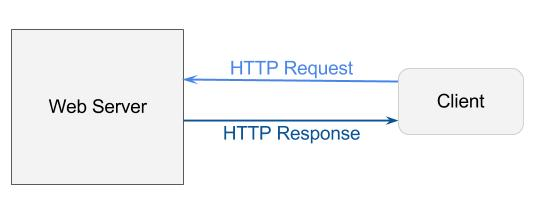
\includegraphics{img/web-server.jpg}}
                    \caption{Model komunikace webového serveru s klientem \cite{webserverVsServletPage}}
                    \label{imgWebserver}
                \end{center}
            \end{figure}

        \subsection{Servlet kontejner}
            Jelikož dostávat stále stejná statická data při stejném požadavku není dostatečná funkcionalita serveru,
            tak existují způsoby jak zajistit dynamickou práci s daty na serveru (a tudíž i měnící se odpovědi na stejný dotaz).
            Jedním ze způsobů jak této činnosti docílit je využití tzv. \emph{servlet kontejneru} a \emph{servletů},
            které jsou navrženy pro programovací jazyk Java.

            Servlet je standardní program (konkrétně jedna třída) napsaný v jazyce Java, 
            který implementuje rozhraní \texttt{javax.servlet}.
            Implementace tohoto rozhraní ho zavazuje k definování několika metod, ale jinak se jedná o běžnou
            třídu z které jsou při zpracovávání požadavků vytvářeny její instance.

            Základní myšlenkou servlet kontejneru je umožnit dynamicky vytvářet odpovědi (často webové stránky)
            pomocí vykonávání servletů. Samotný servlet kontejner je program, který poskytuje běhové prostředí pro vykonávání servletů,
            zajišťuje jejich vytváření, vykonávání a odstraňování. Dále se také podílí na zpracovávání HTTP požadavků, které jsou
            mu předávány od webového serveru. 

            Popsaný způsob fungování servlet kontejneru je znázorněn na obrázku \ref{imgServlet}.
            %teoreticky bych mohl dopsat něco o způsobu vyhodnocení servletu, ale to asi není podstatné
            \begin{figure}[ht]
                \begin{center}
                    \scalebox{0.75}{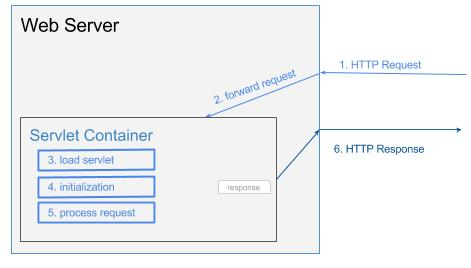
\includegraphics{img/servlet-container-life-cycle.jpg}}
                    \caption{Ukázka způsobu činnosti servlet kontejneru a jeho spolupráce s webovým serverem \cite{webserverVsServletPage}}
                    \label{imgServlet}
                \end{center}
            \end{figure}


         
    \section{Maven} \label{maven}
        Základní obecné informace, něco o pomkách - co tam najdeme, způsobech překladů
        \cite{mavenWeb}

    \section{Winstone} \label{winstone}
        Aspoň základní informace, aby následující kapitola byla lehčeji pochopitelná?

        že je upraven pro Jenkins, puvodne jen trochu a ted jsou jeho streva nahrazena pomoci Jetty
        neuhlazeny kod, plno mrtveho kodu, neni dukladne otestovan, narychlo vymenen

        jak to bylo ve verzi 0.9 a 2.0

        upraveny winstone v jenkins napr. nepodporuje clustorovani, ptoroze byl problem s tim, ze pres session
        promennou predaval hodnoty --->problem se spustenim vice instanci na jedne IP
        \cite{winstoneWeb}

    \section{Jetty} \label{jetty}
        \cite{jettyWeb}
        obecné seznámení, co to umí

    \section{Undertow} \label{undertow}
        Obecné informace, k čemu je dobrý, srovnání s Jetty, odkazy na výsledky testování výkonu

        Jak se používá, jak se s ním pracuje a programuje, detailněji
         argumenty v pdfku k wildfly8 - bezpecnost, rychlost, ...


        \cite{undertowWeb}

        


\chapter{Analýza problému}
    
    \section{Aktuální stav architektury webového serveru a servlet kontejneru v Jenkins CI}
        Popis aktuálního stavu architektury Jenkins z pohledu servlet kontejneru, 
        
        možnosti integrace: napojení Winstone a Jetty v Jenkins
        extras-executebles-war, vkládání winstonu jako .jar

    \section{Zjištěné problémy}
        Rozdílná verze Javy - Undertow v. 7, Jenkins v. 6
        
    \section{Zpětná kompatibilita}
        zachování funkčnosti parametrů - závisí na tom různé komponenty a pluginy Jenkins. 
        Odcitovat Keysukeho čláenk na docs.gmail.       
        
    \section{Varianta ponechání Winstonu}

    \section{Varianta nahrazení Jetty i Winstonu}

    \section{Zvolená varianta}
        Způsob vyhodnocení správnosti výsledného řešení pomocí testů jenkins



\chapter{Závěr}


%=========================================================================



